\chapter{Interpolating with Polynomials}

Let's say someone on a distant planet records video of a hammer being
throw up into the air.  They send you three random frames of the
hammer in flight. Each frame has a timestamp and you can clearly see
how high the hammer is in each one. Can you create a 2nd degree
polynomial that explains the entire flight of the hammer?

That is, you have three points $(t_0, h_0), (t_1, h_1), (t_2, h_2)$.
Can you find $a,b,c$ such that the graph of $at^2 + bt + c = t$ passes
through all three points?

The answer is yes.  In fact, given any $n$ points, there is exactly
one $n-1$ degree polynomial that passes through all the points.

There are a lot of variables floating around. Let's make it concrete:
The photos are taken at $t = 2$ seconds, $t = 3$ seconds, and $t = 4$
seconds. In those photos, the height of the hammer is $5m$, $7m$, and
$6m$. So, we want our polynomial to pass through these points: (2, 5),
(3, 7), (4,6).

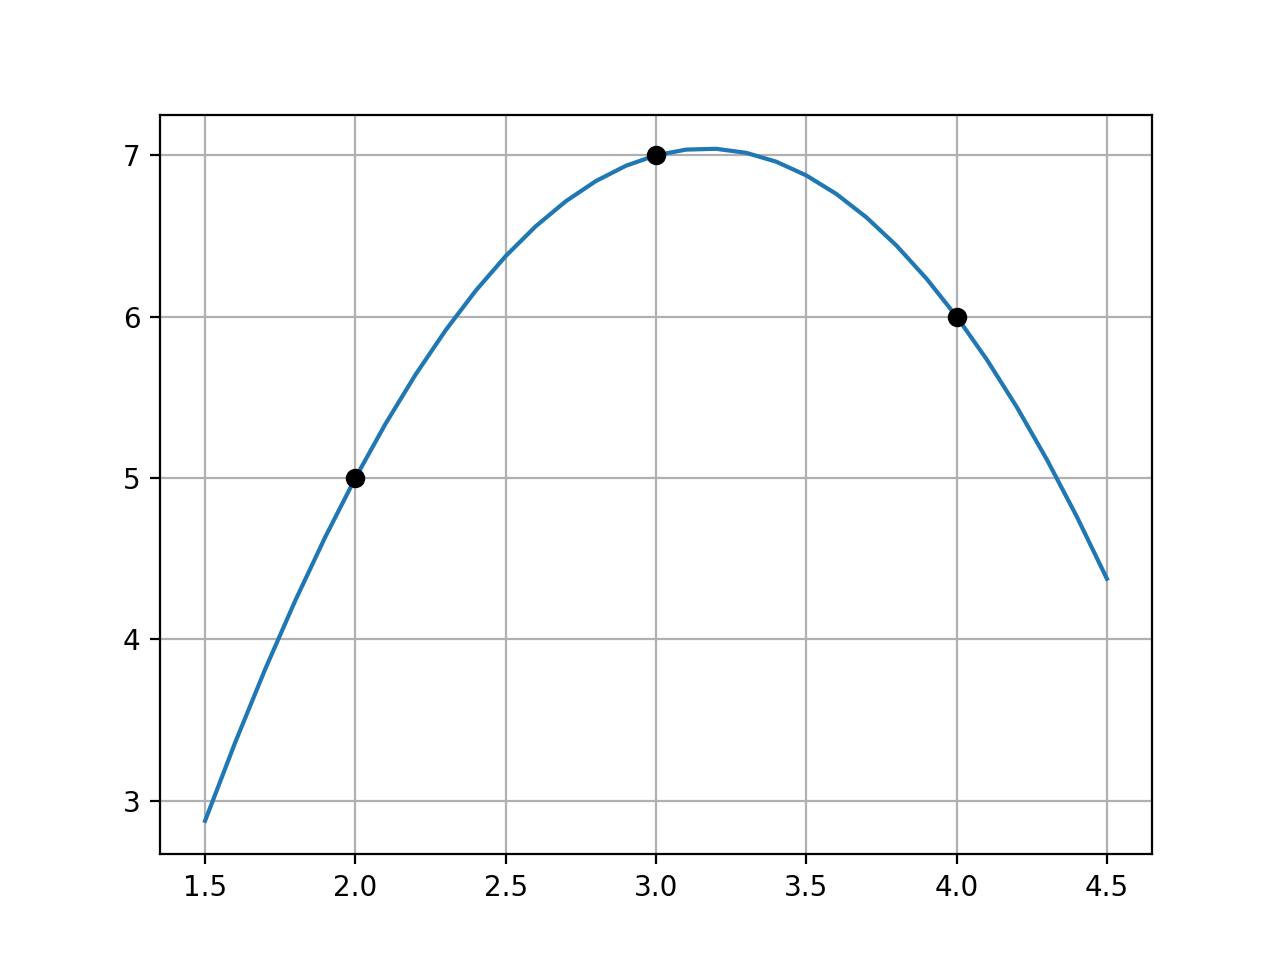
\includegraphics[width=0.5\textwidth]{interpolation.png} 
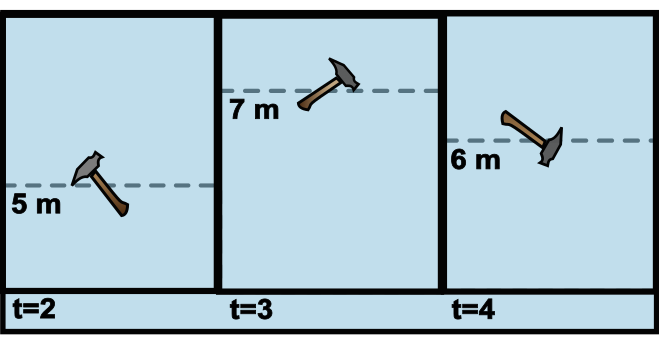
\includegraphics[width=0.5\textwidth]{hammer_1.png}


How can you find that polynomial? Let's do it in small steps. Can you
create a 2nd degree polynomial that is not zero at $t = 2$, but is zero
at $t = 3$ and $t = 4$? Yes, you can: $(x - 3)(x - 4)$ has
exactly two roots at $t = 3$ and $t = 4$.  The value of this polynomial at
$t = 2$ is $(2 - 3)(2 - 4) = 2$. We really want it to be $5m$, so
we can divide the whole polynomial by 2 and multiply it by 5.

Now we have the polynomial:
\begin{equation*}
f_0(x) = \frac{5}{(2 - 3)(2 - 4)}(x - 3)(x - 4) = \frac{5}{2}x^2 - \frac{35}{2}x + 30
\end{equation*}
This is a second degree polynomial that is 5 at $t=2$ and 0 at $t=3$ and $t=4$.

Now we create a polynomial that is 7 at $t=3$ and 0 at $t= 2$ and $t=4$:
\begin{equation*}
f_1(x) = \frac{7}{(3 - 2)(3 - 4)}(x - 2)(x - 4) = -7x^2 +42x - 56
\end{equation*}

Finally, we create a polynomial that is 6 at $t=4$ and zero at $t=2$ and $t=3$:
\begin{equation*}
f_2(x) = \frac{6}{(4 - 2)(4 - 3)}(x - 2)(x - 3) = 3x^2 - 15x + 18
\end{equation*}

Adding these three polynomials together gives you a new polynomial that touches all three points:
\begin{equation*}
  f(x) = \frac{5}{2}x^2 - \frac{35}{2}x + 30  - 7x^2 + 42x - 56 + 3x^2 - 15x + 18  = -\frac{3}{2}x^2 + \frac{19}{2}x -8
\end{equation*}

You can test this with your \pytype{Polynomial} class. Create a file called \filename{test\_interpolation.py}. Add this code:
\begin{Verbatim}
from Polynomial import Polynomial
import matplotlib.pyplot as plt

in_x = [2,3,4]
in_y = [5,7,6]

pn = Polynomial([-8, 19/2, -3/2])
print(pn)

# These lists will hold our x and y values
x_list = []
y_list = []

# Starting x
current_x = 1.5

while current_x <= 4.5:
    # Evaluate pn at current_x
    current_y = pn(current_x)

    # Add x and y to respective lists
    x_list.append(current_x)
    y_list.append(current_y)

    # Move x forward
    current_x += 0.05
    
# Plot the curve
plt.plot(x_list, y_list)

# Plot black circles on the given points
plt.plot(in_x, in_y, "ko")
plt.grid(True)
plt.show()
\end{Verbatim}

You should get a nice plot that shows the graph of the polynomial
passing through those three points.

In general, then, if you give me any three points $(t_0, h_0), (t_1, h_1), (t_2, h_2)$, here is a second degree polynomial that pass through all three points:
\begin{equation*}
\frac{h_0}{(t_0 - t_1)(t_0 - t_2)}(x - t_1)(x - t_2) + \frac{h_1}{(t_1 - t_0)(t_1 - t_2)}(x - t_0)(x - t_2) + \frac{h_2}{(t_2 - t_0)(t_2 - t_1)}(x - t_0)(x - t_1)
\end{equation*}

What if you are given 9 points ($(t_0, h_0), (t_1, h_1), \ldots, (t_8,
h_8)$) and want to find a 8th degree polynomial that passes through
all of them? Just what you would expect:
\begin{equation*}
\frac{h_0}{(t_0 - t_1)(t_0 - t_2)\ldots(t_0 - t_8)}(x - t_1)(x - t_2)\ldots(x - t_8) + \ldots + \frac{h_8}{(t_8 - t_0)\ldots(t_8-t_7)}(x - t_0)\dots(x - t_7)
\end{equation*}

\textit{FIXME: Do I need to define summation and prod here?}

The general solution is, given $n$ points, the $n-1$ degree polynomial that goes through them is
\begin{equation*}
  y =\sum_{i=0}^{n}\left ( \prod_{\stackrel{\!0\leq j\leq n}{j\neq i}}\frac{x-t_j}{t_i-t_j}\right ) h_i
\end{equation*}

That would be tedious for a person to compute, but computers love this
stuff. Let's create a method that creates instances of Polynomial
using interpolation.

\section{Interpolating polynomials in python}

Your method will take two lists of numbers, one contains x-values and
the other contains y-values. So comment out the line that creates the
polynomial in \filename{test\_interpolation.py} and create it from two lists:
\begin{Verbatim}
in_x = [2,3,4]
in_y = [5,7,6]
# pn = Polynomial([-8, 19/2, -3/2])
pn = Polynomial.from_points(in_x, in_y)
print(pn)
\end{Verbatim}

Add the following method to your Polynomial class in \filename{Polynomial.py}
\begin{Verbatim}
    @classmethod
    def from_points(cls, x_values, y_values):
        coef_count = len(x_values)

        # Sums start with a zero polynomial
        sum_pn = Polynomial([0.0] * coef_count)
        for i in range(coef_count):

            # Products start with the constant 1 polynomial
            product_pn = Polynomial([1.0])
            for j in range(coef_count):

                # Must skip j=i
                if j != i:
                    # (1x - x_values[j]) has a root at x_values[j]
                    factor_pn = Polynomial([-1 * x_values[j], 1])
                    product_pn = product_pn * factor_pn
                    
            # Scale so product_pn(x_values[i]) = y_values[i]
            scale_factor  = y_values[i] / product_pn(x_values[i])
            scaled_pn = scale_factor * product_pn

            # Add it to the sum
            sum_pn = sum_pn + scaled_pn
            
        return sum_pn  
\end{Verbatim}

It should work exactly the same as before.  You should get the same
polynomial printed out as before. You shoud get the same plot of the
curve passing through the three points.

How about five points? Change \pyvar{in\_x} and \pyvar{in\_y} at the
start of \filename{test\_interpolation.py}:
\begin{Verbatim}
in_x = [1.7, 2, 2.7, 3.5, 4, 4.4]
in_y = [8, 12, 1, 4, -1, 6]
\end{Verbatim}

You should get a polynomial that passes through all five points:
\begin{equation*}
11.21x^5 - 171.05x^4 + 1019.44x^3 - 2957.53x^2 + 4161.78x - 2258.75  
\end{equation*}
It should look like this:
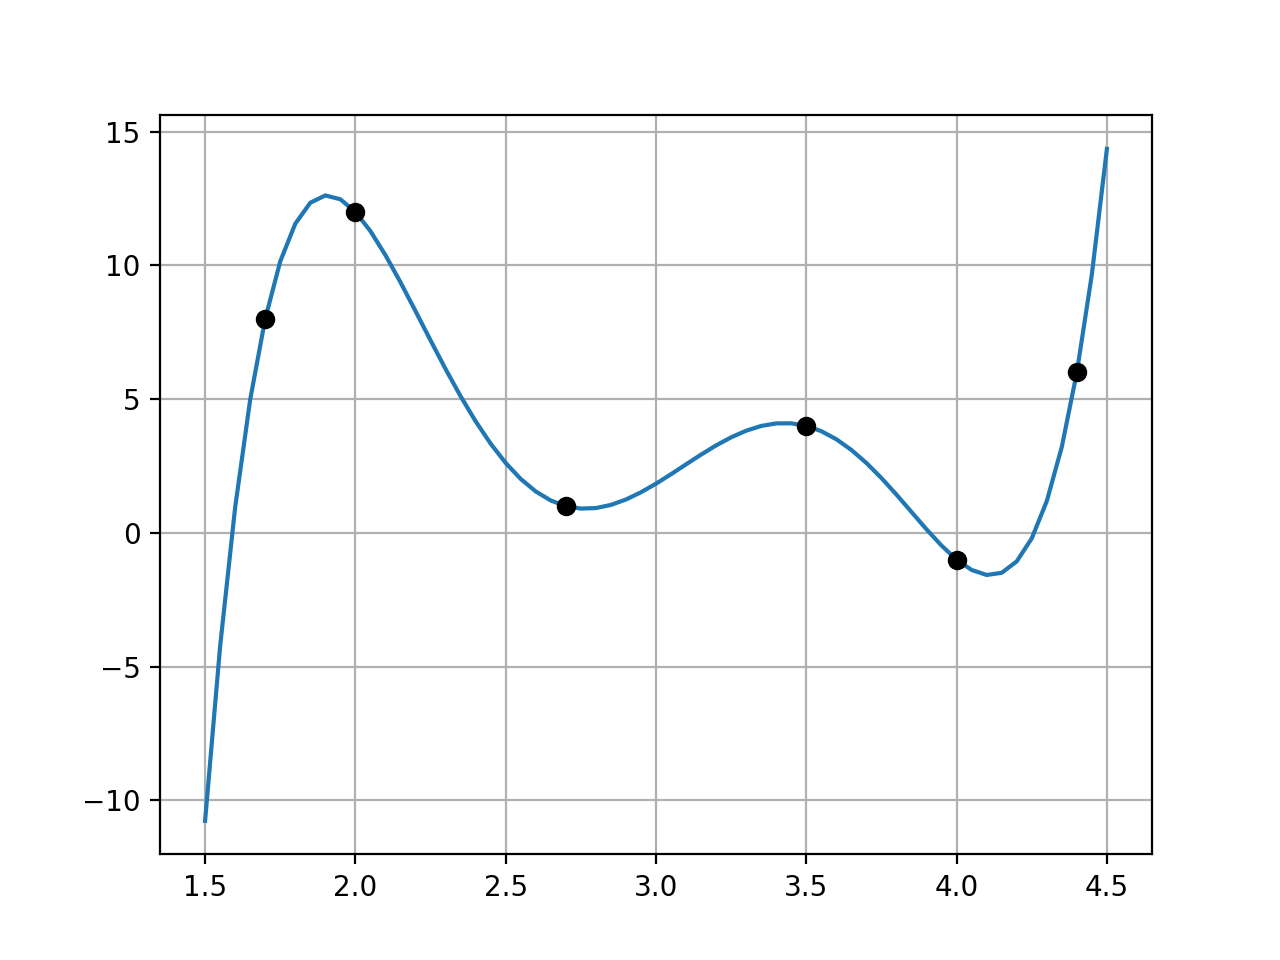
\includegraphics[width=0.7\textwidth]{fiveinterp.png}
